\documentclass[a4paper,oneside,12pt,pdftex]{article}
\usepackage[bahasa]{babel}
\usepackage[top=3cm,left=2.5cm,bottom=3.9cm,right=2.5cm]{geometry}
\usepackage{times}
\usepackage{graphicx}
\usepackage{wrapfig}
\usepackage{subfig}
\usepackage{array}
\usepackage{multirow}
\usepackage{color}
\usepackage{colortbl}
\definecolor{sectioncolor}{rgb}{0.211764706,0.37254902,0.568627451}
\definecolor{subsectioncolor}{rgb}{0.309803922,0.505882353,0.741176471}
\usepackage{hyperref}
\hypersetup{colorlinks,citecolor=blue,filecolor=black,linkcolor=blue,urlcolor=blue,breaklinks=true}
\usepackage{fancyhdr}
\pagestyle{fancy}
\fancyhead{}
\fancyfoot{}
\lfoot
{
\begin{tabular}{|>{\footnotesize}l|}
\hline
\cellcolor[gray]{0.949019608}Nomor Dokumen: IMP\hspace{2cm}Nomor Revisi: 02\hspace{0.7cm}Tanggal: 17/03/10\hspace{1.5cm}Halaman \thepage\hspace{3pt}dari 14\\
\hline
\end{tabular}\\
{\scriptsize\copyright 2010 oleh LSKK STEI-ITB. Pengungkapan dan penggunaan seluruh isi dokumen hanya dapat dilakukan atas ijin tertulis LSKK STEI-ITB Jalan Ganesha 10 Bandung, 40132 Indonesia.}
}
\renewcommand{\headrulewidth}{0pt}


\begin{document}

\addcontentsline{toc}{section}{Lembar Sampul Dokumen}

\begin{wrapfigure}{l}{0.125\textwidth}
\vspace{-0.5cm}

\includegraphics[height=2.6cm]{Ganesha}
%\rule{\linewidth}{0.2mm}
\end{wrapfigure}
\noindent\textbf{\textsf{\LARGE Dokumen Pengembangan Produk}}\\[0.8cm]
\textsf{\large LAB. SISTEM KENDALI \& KOMPUTER, STEI -- ITB}
\rule{\linewidth}{0.2mm}
\vspace{0.5cm}
\begin{center}
\textbf{\textcolor{sectioncolor}{\textsf{\large Lembar Sampul Dokumen}}}\\[1.1cm]
\end{center}

\arrayrulecolor{white}
\setlength\doublerulesep{11pt}

\begin{tabular}{p{4cm}>{\columncolor{backgroundcolor}}p{10.5cm}}
Judul Dokumen & DOKUMEN DESAIN PRODUK:\\[0.1cm]
 & \cellcolor{backgroundcolor}\emph{PUSPA}\\
\hline\hline
\end{tabular}

\begin{tabular}{p{4cm}p{10.5cm}}
Jenis Dokumen & \cellcolor{backgroundcolor}DSG: DESAIN PRODUK\\
 & \hspace{1.25cm}\textmd{\textsf{\scriptsize Catatan: Dokumen ini dikendalikan penyebarannya oleh LSKK, STEI -- ITB}}\\[0.4cm]
\end{tabular}

\begin{tabular}{p{4cm}p{10.5cm}}
Nomor Dokumen & \cellcolor{backgroundcolor}DSG\\
\hline\hline
\end{tabular}

\begin{tabular}{p{4cm}p{10.5cm}}
Nomor Revisi & \cellcolor{backgroundcolor} 02\\
\hline\hline
\end{tabular}

\begin{tabular}{p{4cm}p{10.5cm}}
Nama Berkas & \cellcolor{backgroundcolor}B300.pdf\\
\hline\hline
\end{tabular}

\begin{tabular}{p{4cm}p{10.5cm}}
Tanggal Penerbitan & \cellcolor{backgroundcolor}17 Maret 2010\\
\hline\hline
\end{tabular}

\begin{tabular}{p{4cm}p{10.5cm}}
Unit Penerbit & \cellcolor{backgroundcolor}PUSPA Dev Team\\
\hline\hline
\end{tabular}

\begin{tabular}{p{4cm}p{10.5cm}}
Banyak Halaman & \cellcolor{backgroundcolor}12\\
 & \\[1.1cm]
\end{tabular}

\arrayrulecolor{black}
\setlength\arrayrulewidth{1pt}

\begin{tabular}{|l|l|l|l|l|l|}
\hline
\multicolumn{6}{|l|}{\cellcolor{backgroundcolor}Data Pengusul}\\
\hline
Pengusul & Nama & \multicolumn{2}{l|}{Erik Prabowo} & Jabatan & \textit{Engineer}\\
 & & \multicolumn{2}{l|}{Rio Andita Setiabakti} & & \textit{Engineer}\\
\hline
\multicolumn{2}{|l|}{Tanggal} & \multicolumn{2}{l|}{17 Maret 2010} & Tanda &\\
\multicolumn{2}{|l|}{} & \multicolumn{2}{l|}{} & Tangan &\\
\hline
\multicolumn{2}{|l|}{Lembaga} & \multicolumn{4}{l|}{Rumah Tenda}\\
\multicolumn{2}{|l|}{} & \multicolumn{4}{l|}{Rakreasi}\\
\hline
\multicolumn{2}{|l|}{Alamat} & \multicolumn{4}{l|}{Jln. Ligar Kencana Blok B No. 8 Bandung 40191}\\
\multicolumn{2}{|l|}{} & \multicolumn{4}{l|}{Jln. Tubagus Ismail VIII No. 68 Bandung 40124}\\
\hline
Telepon & {\footnotesize 022-2509262} & Faks & {\footnotesize 022-2509262} & \textit{e-mail} & {\footnotesize\href{mailto:eprabowo@rumahtenda.web.id}{eprabowo@rumahtenda.web.id}}\\
 & {\footnotesize 022-82523428} & & {\footnotesize 022-82523428} & & {\footnotesize\href{mailto:rio.andita@gmail.com}{rio.andita@gmail.com}}\\
\hline
\end{tabular}

\vspace{0.75cm}

\arrayrulecolor{black}
\setlength\arrayrulewidth{0.6pt}

\tableofcontents
\part*{\textcolor{sectioncolor}{\textsf{\large Catatan Sejarah Perbaikan Dokumen}}}
\addcontentsline{toc}{section}{Catatan Sejarah Perbaikan Dokumen}

\begin{tabular}{|p{4cm}|p{11cm}|}
\hline
{\scshape Versi, Tgl, Oleh} & {\scshape Perbaikan}\\
\hline
01, 18 Desember 2009, Erik Prabowo \& Rio Andita Setiabakti & Sebuah dokumen baru yang memaparkan spesifikasi PUSPA.\\
\hline
02, 22 Januari 2010, Erik Prabowo \& Rio Andita Setiabakti & Memperbaharui modul-modul.\\
\hline
03, 17 Maret 2010, Erik Prabowo \& Rio Andita Setiabakti & Memperbaharui setelah mengubah perancangan.\\
\hline
\end{tabular}

\part*{\centering\textsf{\large IMPLEMENTASI PRODUK}}


\section*{\textcolor{sectioncolor}{\textsf{\large PENGANTAR}}}
\addcontentsline{toc}{section}{PENGANTAR}

\subsection*{\textsf{\normalsize 1.1\hspace{0.5cm}RINGKASAN ISI DOKUMEN}}
\addcontentsline{toc}{subsection}{1.1 RINGKASAN ISI DOKUMEN}

Dokumen ini akan memberikan gambaran awal tentang perencanaan pengembangan, analisis pasar, hingga studi kelayakan usaha produksi PUSPA. Kami akan menunjukkan ilustrasi dasar PUSPA berikut konsep rancangannya. Pun dalam dokumen ini kami akan menunjukkan kelayakan usaha produksi PUSPA dengan nilai NPV yang cukup menggiurkan.

\subsection*{\textcolor{subsectioncolor}{\textsf{TUJUAN PENULISAN DAN APLIKASI\slash KEGIATAN}}}
\addcontentsline{toc}{subsection}{TUJUAN PENULISAN DAN APLIKASI\slash KEGIATAN}

Tujuan utama tulisan ini dibuat adalah agar para penulis dokumen ini, yang sedang mengikuti Program Magister Teknik Elektro Opsi Teknologi Media Digital dan Game di ITB, dapat memenuhi salah satu dari persyaratan-persyaratan pembuatan produk yang nantinya akan menjadi bahan tesis.
Tulisan ini ditujukan kepada tim dan pembimbing tesis LSKK STEI--ITB.

Maksud dari penulisan dokumen ini adalah untuk memberikan rincian spesifikasi yang lebih dalam,
yang dari situ akan terlihat lebih jelas juga bagaimana PUSPA dirancang.

\subsection*{\textcolor{subsectioncolor}{\textsf{REFERENSI}}}
\addcontentsline{toc}{subsection}{REFERENSI}
%\begin{itemize}
%\item Han J. Y., \emph{Low-cost multi-touch sensing through frustrated total internal reflection}.\\ 
%  UIST '05: Proceedings of the 18th annual ACM symposium on User Interface Software and Technology, pp. 115-118. ACM, 2005.
%\item Han J. Y., \emph{Multi-touch sensing through frustrated total internal reflection}.\\
%  SIGGRAPH '05: ACM SIGGRAPH 2005 Sketches, pp. 145. ACM, 2005.
%\item Jurafsky D. \& Martin J. H., \emph{Speech and Language Processing}, 2nd ed.\\
%  Upper Saddle River, New Jersey 07458: Pearson Education, Inc., 2009.
%\item Nakatani L. H. \& Rohrlich J. A., \emph{Soft machines: A philosophy of user-computer interface design}.
%  CHI '83: Proceedings of the SIGCHI conference on Human Factors in Computing Systems, pp. 19-23. ACM, 1983.
%\item Poslad S., \emph{Ubiquitous Computing: Smart Devices, Environments and Interactions}.\\
%  Wiley \& Sons, Gebundene Ausgabe, 2009.
%\item Thalmann D., Noser H. \& Huang Z., \emph{Autonomous Virtual Actors Based on Virtual Sensors}, \emph{Creating Personalities for Synthetic Actors}, pp. 25-42, 1997.
%\item Trappl R. \& Petta P. (Eds.), \emph{Creating Personalities for Synthetic Actors: Towards Autonomous Personality Agents}, Vol. 1195. Springer, 1997.
%\item Walker M. A. \& Rambow O., \emph{Computer Speech and Language, Special Issue on Spoken Language Generation}, July 2002.
%\item Wilson A. D., \emph{TouchLight: an imaging touch screen and display for gesture-based interaction}.
%  ICMI '04: Proceedings of the 6th international conference on Multimodal interfaces, pp. 69-76. ACM, 2004.
%\end{itemize}

\subsection*{\textcolor{subsectioncolor}{\textsf{DAFTAR SINGKATAN \& ISTILAH}}}
\addcontentsline{toc}{subsection}{DAFTAR SINGKATAN \& ISTILAH}

\begin{tabular}{|c|c|}
\hline
{\scshape Singkatan} & {\scshape Arti}\\
\hline
3D & 3 Dimensional\\
\hline
CS & ClientSocket (modul)\\
\hline
DM & DialogueManager (modul)\\
\hline
FD & FaceDetector (modul)\\
\hline
GUI & Graphical User Interface\\
\hline
KB & KnowledgeBase (modul)\\
\hline
NLA & NaturalLanguageAnalyser (modul)\\
\hline
NLG & NaturalLanguageGenerator (modul)\\
\hline
NLP & Natural Language Processing\\
\hline
PUSPA & {\scshape Puspa}'s an Understanding Synthespian that Provides Assistance\\
\hline
SR & SpeechRecogniser (modul)\\
\hline
SS & ServerSocket (modul)\\
\hline
SS & SpeechSynthesiser (modul)\\
\hline
ST & Synthespian (modul)\\
\hline
STT & Speech-To-Text\\
\hline
Surel & Surat elektronik\\
\hline
Synthespian & Synthetic thespian\\
\hline
TM & TaskManager (modul)\\
\hline
TTS & Text-To-Speech\\
\hline
UI & UserInterface (modul)\\
\hline
\end{tabular}



\section*{\textcolor{sectioncolor}{\textsf{\large HMT: \textit{HW IMPLEMENTATION \& MODULE TEST SPECIFICATION}}}}
\addcontentsline{toc}{section}{HMT: \textit{HW IMPLEMENTATION \& MODULE TEST SPECIFICATION}}

\subsection*{\textcolor{subsectioncolor}{\textsf{1. \textit{INTRODUCTION}}}}
\addcontentsline{toc}{subsection}{1. \textit{INTRODUCTION}}

Belum ada.

\subsection*{\textcolor{subsectioncolor}{\textsf{2. \textit{LAYOUT}}}}
\addcontentsline{toc}{subsection}{2. \textit{LAYOUT}}

Belum ada.

\subsection*{\textcolor{subsectioncolor}{\textsf{3. \textit{MOUNTING PROCEDURE}}}}
\addcontentsline{toc}{subsection}{3. \textit{MOUNTING PROCEDURE}}

Belum ada.

\subsection*{\textcolor{subsectioncolor}{\textsf{4. \textit{ADJUSTMENT PROCEDURE}}}}
\addcontentsline{toc}{subsection}{4. \textit{ADJUSTMENT PROCEDURE}}

Belum ada.

\subsection*{\textcolor{subsectioncolor}{\textsf{5. \textit{TEST DESCRIPTION}}}}
\addcontentsline{toc}{subsection}{5. \textit{TEST DESCRIPTION}}

Belum ada.

\subsection*{\textcolor{subsectioncolor}{\textsf{6. \textit{TEST REPORT}}}}
\addcontentsline{toc}{subsection}{6. \textit{TEST REPORT}}

Belum ada.



\section*{\textcolor{sectioncolor}{\textsf{\large SMT: \textit{SW IMPLEMENTATION \& MODULE TEST SPECIFICATION}}}}
\addcontentsline{toc}{section}{SMT: \textit{SW IMPLEMENTATION \& MODULE TEST SPECIFICATION}}

\subsection*{\textcolor{subsectioncolor}{\textsf{1. \textit{INTRODUCTION}}}}
\addcontentsline{toc}{subsection}{1. \textit{INTRODUCTION}}

\subsubsection*{ServerSocket \& ClientSocket}
Sebagai percobaan dalam pengembangan tahap awal,
penerapan modul ini mengacu pada program \href{http://beej.us/guide/bgnet/output/html/multipage/clientserver.html}{\textit{stream server} dan \textit{stream client} sederhana pada Hall (2009)},
hanya saja disesuaikan dengan kebiasaan umum pada pemrograman C++.
Secara umum, modul ini berangkat dari sini.
Rencananya, selangkah demi selangkah modul-modul ini akan dilengkapi supaya dapat mewujudkan fitur-fitur yang merupakan bagian dari perancangan PUSPA,
contohnya seperti teknik \textit{synchronous I/O multiplexing}.

\subsubsection*{DialogueManager}
Modul ini merupakan usaha menerapkan \textit{information-state dialogue manager} yang dijelaskan pada Jurafsky \& Martin (2009).
\textit{Dialogue manager} seperti ini diharapkan dapat mengetahui apakah penggunanya sedang bertanya, sedang menyuruh, atau sebagainya.
\textit{Information state}-nya kemudian diperbaharui selagi \textit{dialogue act} pengguna ditafsirkan,
dan \textit{information state} tersebut kemudian akan menjadi parameter dalam menghasilkan \textit{dialogue act} tanggapan.
Beberapa hal yang termasuk dalam \textit{information state} ini mencakup \textit{communicative goal}, \textit{user model}, dan lain-lain.

\subsection*{\textcolor{subsectioncolor}{\textsf{2. \textit{ENVIRONMENT}}}}
\addcontentsline{toc}{subsection}{2. \textit{ENVIRONMENT}}

\subsubsection*{ServerSocket \& ClientSocket}
Bahasa pemrograman yang digunakan adalah C++,
dan pustaka-pustaka yang dibutuhkan mencakup:
\begin{enumerate}
\item Pustaka Standar C;
\item Pustaka POSIX C, terutama Berkeley sockets API;
\item dan Pustaka Standar C++.
\end{enumerate}

\subsubsection*{DialogueManager}
Bahasa pemrograman yang digunakan adalah C++,
dan pustaka-pustaka yang dibutuhkan mencakup:
\begin{enumerate}
\item Pustaka Standar C++;
\item dan PCRE.
\end{enumerate}

\subsection*{\textcolor{subsectioncolor}{\textsf{3. \textit{PROGRAMMING PROCEDURE}}}}
\addcontentsline{toc}{subsection}{3. \textit{PROGRAMMING PROCEDURE}}


\subsubsection*{ServerSocket  \& ClientSocket}

Kode utama yang tercakup dalam modul ServerSocket dan ClientSocket masing-masing dapat ditemukan pada berkas \texttt{ServerSocket.cpp} dan \texttt{ClientSocket.cpp},
yang masing-masingnya memiliki berkas \textit{header}.
Untuk menguji modul-modul ini, telah disediakan juga masing-masing berkas \texttt{serversockettest.cpp} dan \texttt{clientsockettest.cpp}.
Semua kode yang telah disebutkan di atas membutuhkan berkas \texttt{Errors.h} dan \texttt{Errors.cpp} dari direktori \texttt{common} karena sudah mengandung antisipasi terhadap galat.

Pada tahap awal ini,
sambungan yang dibangun masih dibatasi dengan satu \textit{client} saja setiap waktu saja (pada peubah \texttt{backLog}).

Pertama, alamat dan port \textit{server} ditentukan pada kedua modul,
informasi tentang alamatnya didapatkan melalui fungsi \texttt{getaddrinfo(2)},
dan masing-masing modul membuat soket dengan fungsi \texttt{socket(2)}.
Khusus untuk modul ServerSocket,
soketnya dihubungkan dengan \textit{port} lokal yang telah ditentukan sebelumnya,
dengan fungsi \texttt{bind(2)}.
Soket ini akan menjadi soket sambungan.
Setelah itu ServerSocket mulai mendengarkan dengan fungsi \texttt{listen(2)} sampai ada permintaan sambungan dari \textit{client}.
ClientSocket akan meminta sambungan pada \textit{server} dengan fungsi \texttt{connect(2)},
dan ServerSocket akan menerima permintaan tersebut dengan fungsi \texttt{accept(2)},
dan mengerahkan soket baru untuk komunikasi.
Setelah ini selesai, \textit{client} mulai dapat berkomunikasi dengan \textit{server},
yang dilakukan melalui \textit{method} \texttt{receive} dan \texttt{send} pada tiap modul,
yang masing-masingnya merupakan pembungkus dari fungsi \texttt{recv(2)} dan \texttt{send(2)}.

Demi kejelasan,
untuk meng-\textit{compile} kode yang dibutuhkan untuk pengujian modul ServerSocket,
dari dalam direktori \texttt{server},
perintah-perintah \textit{shell}-nya dapat dipaparkan sebagai berikut.
\begin{enumerate}
\item \verb!g++ -I../common -c ../common/Errors.cpp!
\item \verb!g++ -I../common -c ServerSocket.cpp!
\item \verb!g++ -I../common -c serversockettest.cpp!
\end{enumerate}
Dari sini, ada 3 berkas objek yang dihasilkan,
yaitu \texttt{Errors.o}, \texttt{ServerSocket.o}, dan \texttt{serversockettest.o}.

Begitu juga dengan modul ClientSocket,
yang dari dalam direktori \texttt{client},
perintah-perintah \textit{shell}-nya adalah
\begin{enumerate}
\item \verb!g++ -I../common -c ../common/Errors.cpp!
\item \verb!g++ -I../common -c ClientSocket.cpp!
\item \verb!g++ -I../common -c clientsockettest.cpp!
\end{enumerate}
yang menghasilkan \texttt{Errors.o}, \texttt{ClientSocket.o}, dan \texttt{clientsockettest.o}.

Untuk me-\textit{link} berkas-berkas tersebut,
perintah yang diketikkan adalah\\
\verb!g++ Errors.o ServerSocket.o serversockettest.o -o serversocket!\\
yang akan menghasilkan berkas \textit{executable} bernama \texttt{serversocket}, dan\\
\verb!g++ Errors.o ClientSocket.o clientsockettest.o -o clientsocket!\\
yang akan menghasilkan \texttt{clientsocket}.

Sebuah Makefile (dan juga berkas proyek Xcode) disediakan untuk kenyamanan dalam melalui proses-proses di atas dengan sekali perintah.

Untuk men-\textit{debug},
perintah yang diketikkan adalah \verb!./serversocket! dalam direktori \texttt{server},
dan \verb!./clientsocket! dalam direktori \texttt{client}.


\subsubsection*{DialogueManager}
\hyphenation{men-da-pat-kan di-mo-del-kan}

Kode utama modul ini dapat ditemukan pada berkas \texttt{DialogueManager.cpp} beserta \textit{header}-nya.
Modul ini berkaitan dengan pelaksanaan tugas,
yang nantinya akan dilaksanakan oleh modul TaskManager.
Karena pemenuhan prasyarat-prasyarat pelaksanaan tersebut terkandung dalam percakapan,
pemodelan objek tugas dilakukan pada modul ini.
Dalam pengujiannya, satu kelas tugas sudah tersedia, yaitu tugas membuat surel,
yang kodenya ada pada berkas \texttt{Email.cpp} beserta \textit{header}-nya.
Untuk menguji modul ini, telah disediakan juga berkas \texttt{dialoguemanagertest.cpp}.

Pertama, masukan bagi modul ini yang berupa \textit{dialogue act} ditafsirkan untuk mendapatkan jenisnya dan makna yang terkandung dalam kalimatnya.
Ada tiga dasar dalam menentukan jenis suatu \textit{dialogue act},
yaitu tata bahasa, nada bicara, dan susunan percakapan.
Bagaimanapun, pada tahap awal ini, hanya yang pertama yang sudah mulai diterapkan.
Setelah jenis \textit{dialogue act} pengguna dilacak,
modul ini berusaha untuk menentukan \textit{communicative goal} apa yang diinginkan untuk tercapai dalam percakapan yang sedang berlangsung.
Dalam suatu percakapan, mungkin terdapat lebih daripada satu \textit{communicative goal},
oleh karena itu hal ini dimodelkan dengan \textit{container} pada C++.
Dalam tahap awal, jenis \textit{container} yang dipilih adalah \texttt{stack},
dengan anggapan bahwa \textit{communicative goal} yang terakhir muncul harus dicapai sebelum \textit{communicative goal} yang muncul sebelumnya dapat tercapai.
\textit{Communicative goal} tidak muncul pada setiap \textit{dialogue act},
oleh karena itu modul ini harus melakukan pengolahan juga untuk menentukan apakah ada \textit{communicative goal} yang muncul atau tidak.
Jika ada, maka \textit{communicative goal} tersebut akan ditambahkan ke tumpukan (\textit{stack}) \textit{communicative goals}.
Setelah itu, modul ini akan mulai membuat \textit{dialogue act} tanggapannya,
dengan membuat apa yang disebut sebagai \textit{adjacency pairs}.
Modul ini akan menentukan jenis \textit{dialogue act} apa saja yang cocok dijadikan pasangan bagi jenis \textit{dialogue act} masukan dari pengguna,
yang kemudian kemungkinannya dipersempit lagi dengan menggunakan \textit{information state} sebagai parameter.
Di sinilah modul ini akan menentukan hal seperti apakah PUSPA harus menanyakan tentang suatu informasi kepada pengguna untuk dapat melaksanakan suatu tugas,
dan juga akan melakukan hal-hal yang perlu seperti membuat \textit{instance} dari kelas yang berkaitan dengan tugas yang harus dilaksanakan tersebut (dalam pengujian ini, kelas \texttt{Email}).
Setelah itulah baru modul ini dapat menentukan ``isi'' dari tanggapan yang akan dikeluarkan.

Untuk meng-\textit{compile} kode yang dibutuhkan untuk pengujian modul DialogueManager,
dari dalam direktori \texttt{server},
perintah-perintah \textit{shell}-nya adalah
\begin{enumerate}
\item \verb!g++ -c Email.cpp!
\item \verb!g++ -c DialogueManager.cpp!
\item \verb!g++ -c dialoguemanagertest.cpp!
\end{enumerate}
yang menghasilkan \texttt{Email.o}, \texttt{DialogueManager.o}, dan \texttt{dialoguemanagertest.o}.

Untuk me-\textit{link} berkas-berkas tersebut,
perintah yang diketikkan adalah
\begin{verbatim}
g++ -lpcrecpp Email.o DialogueManager.o dialoguemanagertest.o \
-o dialoguemanager
\end{verbatim}
yang akan menghasilkan \texttt{dialoguemanager}.

Untuk men-\textit{debug},
perintah yang diketikkan adalah \verb!./dialoguemanager! dalam direktori \texttt{server}.

\subsection*{\textcolor{subsectioncolor}{\textsf{4. \textit{TEST DESCRIPTION}}}}
\addcontentsline{toc}{subsection}{4. \textit{TEST DESCRIPTION}}


\subsubsection*{ServerSocket \& ClientSocket}

Konteks pengujian pada kedua modul ini adalah untuk membuktikan bahwa komunikasi antara subsistem \textit{server} dengan \textit{client} sudah dapat berjalan dengan lancar dan mapan.
Oleh karena itu,
antarmuka yang disediakan untuk pengujian ini cukup berupa konsol untuk memasukkan teks di sisi \textit{client} yang kemudian akan dikirim ke \textit{server},
dan sesampainya di \textit{server},
teks tersebut hanya akan dikembalikan lagi tanpa diolah terlebih dahulu.

Yang diuji dari ServerSocket adalah kemampuannya menyalakan layanan dan menunggu sampai ada \textit{client} dari manapun yang mencoba membuat sambungan dengan \textit{server},
kemampuannya mengenali informasi alamat \textit{client},
kemampuannya membuat \textit{server} berkomunikasi dengan satu \textit{client} tersebut setelah itu,
kemampuannya untuk membuat \textit{server} kembali menunggu setelah \textit{client} tersebut keluar dari sambungannya,
dan kemampuannya untuk mengulangi proses-proses tersebut ketika ada \textit{client} yang menyambung lagi.

Yang diuji dari ClientSocket adalah kemampuannya menyambung ke \textit{server},
kemampuannya mengenali \textit{server},
dan kemampuan untuk berkomunikasi dengannya.

Semua pengujian yang disebutkan di atas dilakukan pada jaringan yang keadaannya mapan.
Apa yang akan terjadi kalau keadaan jaringannya tidak mapan,
sebenarnya dapat juga diketahui hanya dengan simulasi.
Bagaimanapun, hal ini belum diuji karena akan memakan waktu yang tidak sebentar,
sedangkan masih banyak hal dalam pengembangan PUSPA yang harus didahulukan.

Masukan pada pengujian ini berupa teks seperti apa saja,
hanya saja karakter dengan banyak lebih daripada 100 tidak diharapkan,
karena penyangga yang disediakan di kedua modul hanya segitu besarnya (tanpa alasan tertentu).
Hal ini belum terlalu dipikirkan,
karena pada pelaksanaannya nanti memang karakter yang banyak sebagai masukan tidak diharapkan,
dan kemungkinan besar juga akan dibatasi oleh pemanfaatan bentuk suara, dan bukan teks, sebagai masukan (dan juga keluaran).
Keluaran pada pengujian ini juga berupa teks.

Peralatan perangkat keras pengujiannya melibatkan dua buah komputer.
Komputer pertama, bertindak sebagai server,
dan komputer kedua, bertindak sebagai client.
Konfigurasi pada pengujian ini adalah kedua komputer tersebut berada dalam satu LAN,
komputer \textit{server} dikenal dengan nama \texttt{rumahtenda.web.id},
dan \textit{port} yang digunakan adalah \textit{port} 12110.
Oleh karena itu, pada jaringannya harus dipastikan bahwa \textit{port} tersebut tidak terhalang.
Versi IP yang digunakan tidak ditentukan, sehingga dapat berupa versi 4 atau 6.
Untuk kenyamanan pengambilan gambar,
pada \textit{server}, peralatan perangkat lunaknya adalah \textit{server} SSH,
sedangkan pada \textit{client}, peralatannya mencakup \textit{client} SSH dan emulator terminal.
Hal ini dilakukan agar ServerSocket dapat dijalankan dari komputer \textit{client},
sehingga kedua modul dapat dijalankan dari satu komputer.
Untuk menjalankan ClientSocket, peralatan perangkat lunak yang dibutuhkan hanya emulator terminal.
Gambar \ref{ServerSocketConfiguration} menunjukkan konfigurasi pada \textit{server},
sedangkan Gambar \ref{ClientSocketConfiguration} menunjukkan konfigurasi pada \textit{client}.

\begin{figure}
\centering
\subfloat[\textit{Server}]{\label{ServerSocketConfiguration}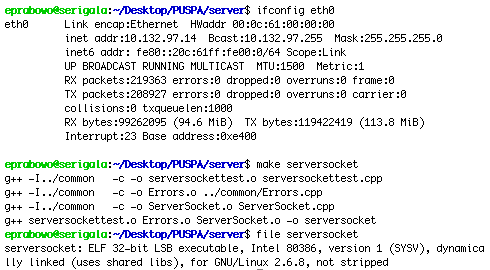
\includegraphics[width=0.5\textwidth]{ServerSocketConfiguration}}
\subfloat[\textit{Client}]{\label{ClientSocketConfiguration}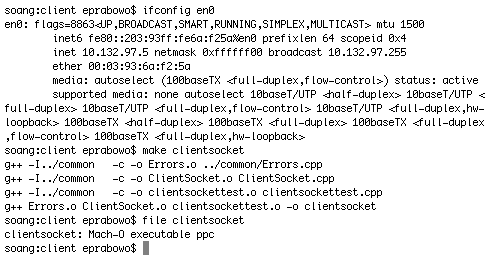
\includegraphics[width=0.5\textwidth]{ClientSocketConfiguration}}
\caption{Konfigurasi ServerSocket dan ClientSocket}
\label{SocketConfiguration}
\end{figure}

Hasil yang diharapkan dari pengujian ini adalah kedua modulnya dapat dengan lancar saling mengirim dan menerima data karakter,
dapat saling mengenali dengan baik melalui informasi mengenai alamat masing-masingnya,
dan kerja tiap modulnya tidak saling terpengaruhi oleh yang lain di saat salah satu memutuskan sambungan yang sudah terbangun.

Pengujian pertama adalah pengujian yang menyebabkan tidak adanya proses yang dilaksanakan.
Hal ini dapat dicapai dengan menyalakan hanya satu subsistem saja.
Gambar \ref{ServerSocketDegenerate} menunjukkan jalannya \textit{server} tanpa \textit{client},
sedangkan Gambar \ref{ClientSocketDegenerate} menunjukkan jalannya \textit{client} tanpa \textit{server}.

\begin{figure}
\centering
\subfloat[\textit{Server} tanpa \textit{client}]{\label{ServerSocketDegenerate}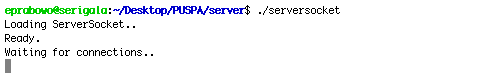
\includegraphics[width=0.5\textwidth]{ServerSocketDegenerate}}
\subfloat[\textit{Client} tanpa \textit{server}]{\label{ClientSocketDegenerate}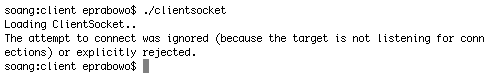
\includegraphics[width=0.5\textwidth]{ClientSocketDegenerate}}
\caption{\textit{Degenerate cases} pada ServerSocket dan ClientSocket}
\label{SocketDegenerate}
\end{figure}

Pengujian kedua adalah pengujian dengan memberikan nilai-nilai batas.
Satu hal yang masih memiliki nilai batas adalah penyangga yang digunakan untuk menampung karakter-karakter yang diterima melalui soket.
Pengujian ini dapat dilakukan dengan memberi masukan karakter yang banyaknya lebih daripada 100.
Gambar \ref{ServerSocketBoundary} menunjukkan \textit{server} saat menerima karakter-karakter yang banyak,
sedangkan Gambar \ref{ClientSocketBoundary} menunjukkan \textit{client} karakter-karakter banyak tersebut ketika dikirim dan ketika diterima kembali.

\begin{figure}
\centering
\subfloat[\textit{Server} menerima banyak karakter]{\label{ServerSocketBoundary}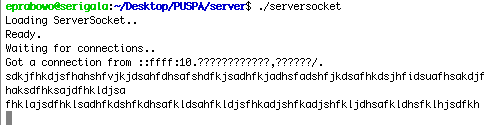
\includegraphics[width=0.5\textwidth]{ServerSocketBoundary}}
\subfloat[\textit{Client} mengirim banyak karakter]{\label{ClientSocketBoundary}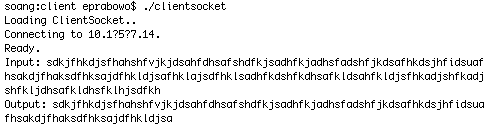
\includegraphics[width=0.5\textwidth]{ClientSocketBoundary}}
\caption{\textit{Boundary cases} pada ServerSocket dan ClientSocket}
\label{SocketBoundary}
\end{figure}

Pengujian ketiga adalah pengujian dengan memberikan data normal.
Gambar \ref{ServerSocketNonUnique} dan Gambar \ref{ClientSocketNonUnique} masing-masing menunjukkan \textit{server} dan \textit{client} saat menerima data normal.

\begin{figure}
\centering
\subfloat[\textit{Server} menerima data normal]{\label{ServerSocketNonUnique}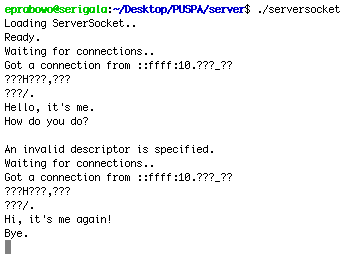
\includegraphics[width=0.5\textwidth]{ServerSocketNonUnique}}
\subfloat[\textit{Client} mengirim data normal]{\label{ClientSocketNonUnique}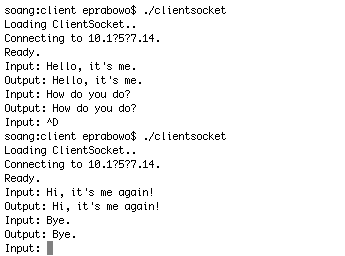
\includegraphics[width=0.5\textwidth]{ClientSocketNonUnique}}
\caption{\textit{Non-unique cases} pada ServerSocket dan ClientSocket}
\label{SocketNonUnique}
\end{figure}


\subsubsection*{DialogueManager}

Konteks pengujian pada modul ini adalah untuk membuktikan bahwa hubungan antara masukan dari pengguna dengan tanggapan yang dikeluarkan oleh modul ini sudah menyimulasikan suatu percakapan.
Di samping itu, pengujian ini juga sudah mulai mempertunjukkan pemenuhan prasyarat suatu pelaksanaan tugas,
walaupun pelaksanaannya belum dapat dilakukan karena hal tersebut merupakan tugas modul TaskManager.
Antarmuka yang disediakan untuk pengujian ini cukup berupa konsol untuk memasukkan teks dan keluarannya juga berupa teks.
Karena modul NaturalLanguageAnalyser yang mengolah bahasa manusia menjadi perwakilan makna untuk diolah oleh modul ini belum mapan,
dan karena modul NaturalLanguageGenerator yang harus mengolah tanggapan yang dihasilkan oleh modul ini menjadi bahasa manusia belum dikerjakan,
masukan dan keluaran modul ini untuk sementara masih dalam bentuk bahasa manusia.

Yang diuji dari modul ini adalah kemampuannya memberikan tanggapan yang cocok dengan masukan yang pengguna berikan,
kemampuannya menentukan \textit{communicative goals} dari percakapan yang sedang berlangsung,
dan kemampuannya melibatkan pengguna dalam pelaksanaan tugas yang diberikan oleh pengguna sendiri dengan cara menanyakan bagaimana pengguna menginginkan tugasnya dilaksanakan.

Yang belum diuji dari modul ini adalah pemeriksaan apakah masukan yang diberikan pengguna itu betul atau tidak dalam konteks percakapan yang sedang berlangsung.
Misalnya ketika pengguna ditanyakan mengenai suatu alamat surel,
jawaban yang diberikan pengguna belum diperiksa apakah betul atau tidak sebagai suatu alamat surel.

Masukan dan keluaran pada pengujian ini berupa teks,
dan banyaknya karakter yang dimasukkan tidak dibatasi.
Peralatan pengujiannya mencakup sebuah komputer dan sebuah emulator terminal.
Hasil yang diharapkan dari pengujian ini adalah simulasi percakapan.

Pengujian pertama adalah pengujian yang menyebabkan tidak adanya proses yang dilaksanakan.
Hal ini dapat dicapai dengan memberikan masukan berupa kata yang tidak diketahui maknanya oleh modul ini.
Gambar \ref{DialogueManagerDegenerate} menunjukkan pengujian ini.

\begin{figure}
\centering
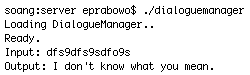
\includegraphics[width=0.5\textwidth]{DialogueManagerDegenerate}
\caption{\textit{Degenerate cases} pada DialogueManager}
\label{DialogueManagerDegenerate}
\end{figure}

Pengujian kedua adalah pengujian dengan memberikan data normal.
Gambar \ref{DialogueManagerNonUnique} menunjukkan simulasi percakapan yang dihasilkan saat yang dimasukkan adalah data normal.

\begin{figure}
\centering
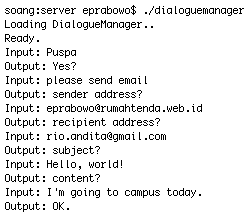
\includegraphics[width=0.5\textwidth]{DialogueManagerNonUnique}
\caption{\textit{Non-unique cases} pada DialogueManager}
\label{DialogueManagerNonUnique}
\end{figure}

\subsection*{\textcolor{subsectioncolor}{\textsf{5. \textit{TEST REPORT}}}}
\addcontentsline{toc}{subsection}{5. \textit{TEST REPORT}}


\subsubsection*{ServerSocket \& ClientSocket}

Kembali pada Gambar \ref{SocketDegenerate},
yang terjadi saat \textit{server} dijalankan tetapi \textit{client} tidak dijalankan adalah \textit{server} tetap menunggu, yang sebenarnya adalah kejadian yang bukan merupakan galat.
Di lain pihak, yang terjadi saat \textit{client} dijalankan tetapi \textit{server} tidak dijalankan adalah program \textit{client} langsung berhenti karena tidak banyak yang \textit{client} dapat lakukan tanpa \textit{server}.

Kembali pada Gambar \ref{SocketBoundary},
yang terjadi saat karakter yang banyak melebihi ukuran penyangga yang tersedia di \textit{server} adalah terpotongnya data yang diterima.
Ternyata datanya diterima semua, hanya setelah dikirim kembali ke \textit{client},
yang diterima hanya potongan pertama.

Kembali pada Gambar \ref{SocketNonUnique},
jika datanya bersifat normal maka tidak ada galat yang muncul yang bersangkutan dengan pengiriman dan penerimaan data.

Walaupun sudah dapat berjalan dan diandalkan,
masih terdapat \textit{bug} yaitu penampilan alamat IP yang tidak betul.
Terlihat pada Gambar \ref{ClientSocketBoundary} dan Gambar \ref{ClientSocketNonUnique},
alamat IPv4 \textit{server} yang ditampilkan pada \textit{client} sudah hampir betul,
hanya bagian tengahnya yang tidak terbaca.
Di lain pihak, seperti terlihat pada Gambar \ref{ServerSocketBoundary} dan Gambar \ref{ServerSocketNonUnique},
alamat IPv6 \textit{client} yang ditampilkan pada \textit{server} sama sekali tidak mendekati.

Yang disarankan sebagai perbaikan pada ServerSocket adalah kemampuan membuat sambungan dan berkomunikasi dengan lebih daripada satu \textit{client},
kemampuan untuk melakukan pengiriman tanpa harus berpasangan dengan penerimaan terlebih dahulu atau sebaliknya,
dan kemampuan mengumumkan layanannya dengan \textit{zeroconf}.

Sama seperti ServerSocket, hal pertama yang disarankan sebagai perbaikan pada ClientSocket adalah kemampuan untuk melakukan pengiriman tanpa harus berpasangan dengan penerimaan terlebih dahulu atau sebaliknya.
Di samping itu, melengkapi saran untuk ServerSocket berkenaan dengan \textit{zeroconf},
ClientSocket disarankan memiliki kemampuan merambah layanan yang diumumkan \textit{server} dengan \textit{zeroconf},
dan menyerahkan keputusan kepada pengguna apakah akan menyambung ketika layanannya ditemukan atau apakah akan keluar dari program ketika layanannya tidak ditemukan.


\subsubsection*{DialogueManager}

Kembali pada Gambar \ref{DialogueManagerDegenerate},
yang terjadi saat masukan yang diberikan maknanya tidak dimengerti oleh modul ini adalah dinyatakannya bahwa PUSPA tidak mengerti apa yang dimaksud oleh pengguna,
yang merupakan tanggapan \textit{default}.

Kembali pada Gambar \ref{DialogueManagerNonUnique},
jika datanya bersifat normal maka hasilnya dapat berupa suatu percakapan yang memiliki tujuan tertentu,
walaupun kalimat yang dimasukkan dan dihasilkan masih terbatas karena belum digunakannya dua modul pendukung modul ini,
yaitu NaturalLanguageAnalyser dan NaturalLanguageGenerator.

Yang disarankan sebagai perbaikan pada modul ini adalah kemampuan menghubungkan setiap masukan dengan konteks percakapan,
misalnya jika pengguna langsung menyuruh tanpa menyapa terlebih dahulu,
maka modul ini akan memastikan dahulu apakah pengguna sedang berbicara dengan PUSPA.
Saran berikutnya adalah pemeriksaan akan sah atau tidaknya masukan pengguna.
Saran terakhir untuk saat ini adalah penerapan unsur-unsur lain dalam \textit{information state},
seperti \textit{user model},
misalnya dengan membuat PUSPA akan menuruti permintaan hanya jika penggunanya memiliki wewenang,
yang tentu saja modul ini harus dapat mengenali penggunanya terlebih dahulu dengan suatu autentikasi.



\appendix
\addcontentsline{toc}{section}{LAMPIRAN}


\end{document}
